When studying gravitational waves, one has to keep in mind that gravitational wave sources (like black hole mergers, neutron stars, etc.) are usually located billions of light years away from us. From the point of view of an observer on Earth, this distance is so vast that it can be approximated as being at infinity. This distance, however, is not sufficiently far away to require accounting for the cosmological constant, allowing us to model spacetime as asymptotically flat. Thus, we are interested in studying the behavior of the gravitational fields at null infinity, $\mathscr{I}$.

To do so, we must perform a conformal compactification of the spacetime, which brings $\mathscr{I}$ to a finite distance on our computational grid. This is done by working in the hyperboloidal coordinate system.

\subsection{Hyperboloidal Coordinates}

The hyperboloidal coordinate system, as previously mentioned, maps our previously unbonded domain to a finite one. This is done by introducing new time and radial coordinates $(t,r)$, which are related to the spherical coordinates of Minkowski spacetime $(T,R)$ by the transformations

\begin{equation}
    \begin{array}{c c} 
        t = T - H(R) & R = \frac{r}{\Omega(r)} \; ,
    \end{array} \; 
\end{equation}
%
where $H(R)$ is called the height function and $\Omega(r)$ is called the compress function, which give rize to the following Jacobian matrix:

\begin{equation}
    \left(J^{Hyp}\right)_{\alpha'}^{\ \ \beta} = 
    \begin{pmatrix}
        1 & -H'(r) & 0 & 0 \\
        0 & \frac{L(r)}{\Omega^2(r)} & 0 & 0 \\
        0 & 0 & 1 & 0 \\
        0 & 0 & 0 & 1
    \end{pmatrix} \; ,
\end{equation}
%
where $H'(r)$ denotes the derivative of the height function with respect to $R$ written as a function of $r$, and $L(r)$ is defined as
%
\begin{equation}
    L(r) \equiv \Omega(r) - r \, \partial_r \Omega(r) \; .
\end{equation}

This coordinate system is particularly useful because it is possible for us to choose the height and compress functions in such a way that the outgoing light speed is constant. This however has the tradeoff of making the incoming light speed decrease as it reaches $\mathscr{I}$. This property can be observed in figure \ref{fig:Good_Speeds} for a specific choice of the height and compress functions.

\begin{figure}[h]
    \centering
    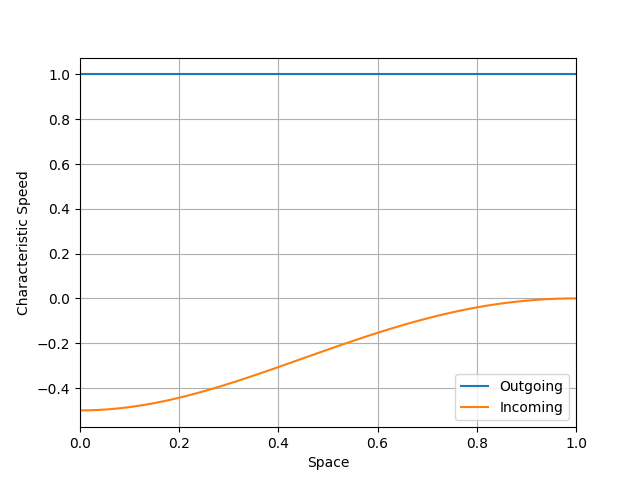
\includegraphics[width=0.5\textwidth]{Images/Good_Speeds.png}
    \caption{Outgoing and incoming light speeds for $H(R) = \frac{2 R^2 + S^2 - \sqrt{4 R^2 S^2 + S^4}}{2R}$ and $\Omega(r) = 1 - \frac{r^2}{S^2}$, with $S = 1$.}
    \label{fig:Good_Speeds}
\end{figure}

Throughout this work, we will sacrifice this very relevant property in exchange for ease of manipulation of the expressions, since the goal of this introductory work to the subject is to get accostumed with the coordinate system. The height and compress functions that will used throughout this work are
%
\begin{equation}
    \begin{array}{c c}
        H(R) = \sqrt{S^2+R^2} & \Omega(r) = \frac{1}{2} \left(1 - \frac{r^2}{S^2}\right)
    \end{array} \; ,
\end{equation}
%
where $S$ is a constant that determines the size of the compactified domain. The choice of $S$ is arbitrary, as it simply defines what point $\mathscr{I}$ will be maped to. We will set $S = 1$. As a consequence of our previous choices, we also have
%
\begin{equation}
    \begin{array}{c c}
        H'(r) = \frac{2 \, r \, S}{S^2 + r^2} & L(r) = \frac{1}{2} \left(1 + \frac{r^2}{S^2}\right) \; .
    \end{array}
\end{equation}

For this choice of functions, we still have that the incoming light speed decreases as it reaches $\mathscr{I}$. However, we don't have a constant outgoing propagation speed. This can be seen in figure \ref{fig:Bad_Speeds}. The only implication this choice will have in our results is that the wave will take longer to reach $\mathscr{I}$ and will be slightly distorted. This is not a problem for our purposes, since on this first approach we are only interested in making sure the code converges smoothly towards the solution.

\begin{figure}[h]
    \centering
    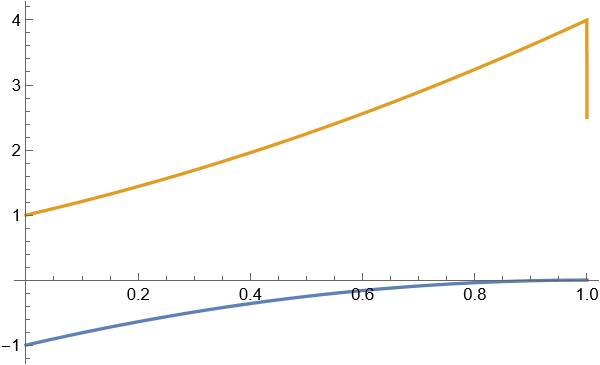
\includegraphics[width=0.5\textwidth]{Images/Bad_Speeds.png}
    \caption{Outgoing and incoming light speeds for $H(R) = \sqrt{S^2+R^2}$ and $\Omega(r) = \frac{1}{2} \left(1 - \frac{r^2}{S^2}\right)$, with $S = 1$.}
    \label{fig:Bad_Speeds}
\end{figure}

\subsection{Computational Setup}

This work is a continuation of my previous work on numerical relativity. As such, the framework used here is the same as the one used in that work, with the adition of truncation error matching for the derivatives, interpolation at the boundaries and the Evans Method for regularization at the origin. The description of the base code can be found in \cite{}, and this section will elaborate on the upgrades made.

\subsubsection{Truncation Error Matching}

Truncation error matching is a technique used to improve the accuracy of the numerical solution by matching the truncation error of the finite difference scheme used on the boundaries to the truncation error of the one used in the interior of our computational domain. This is done by using a one sided finite difference scheme on the boundaries such that the leading order error term is the same as the one used in the interior.

In our framework, we use the following second order finite difference scheme for the first derivative of a field $\psi$ at an interior point $i$ (where the leading order error term was written explicitly):

\begin{equation}
    \psi'_i = \frac{\psi_{i+1} - \psi_{i-1}}{2h} - \frac{h^2}{6} \psi'''_i + ...\; ,
\end{equation}
%
where $\psi_{i+1}$ and $\psi_{i-1}$ are the values of the field $\psi$ at the points $i+1$ and $i-1$ respectively, and $h$ is the grid spacing.

To match this leading order term of the error, we use the following one sided finite difference scheme for the derivative of $f$ at the left and right boundary points respectively \cite{}:

\begin{equation}
    \psi'_i = \frac{\psi_{i+3} - 4 \psi_{i+2} + 7 \psi_{i+1} - 4 \psi_{i}}{2h} - \frac{h^2}{6} \psi'''_i + ...\;
\end{equation}

\begin{equation}
    \psi'_i = \frac{4 \psi_{i} - 7 \psi_{i-1} + 4 \psi_{i-2} - \psi_{i-3}}{2h} - \frac{h^2}{6} \psi'''_i + ...\;
\end{equation}

\subsubsection{Interpolation at the Boundaries}

Since we are interested in evolving the fields at null infinity, we must choose a boundary condition that allows the fields to freely propagate outwards. To do so, we use interpolation at the outer boundaries of our computational domain to fill the ghost points in those regions. This is done by using the following interpolation scheme:

\begin{equation}
    \psi_i = 4 \psi_{i-1} - 6 \psi_{i-2} + 4 \psi_{i-3} - \psi_{i-4} \; ,
\end{equation}
%
where $\psi_i$ is the value of the field at the ghost point $i$, and $\psi_{i-1}$, $\psi_{i-2}$, $\psi_{i-3}$ and $\psi_{i-4}$ are the values of the field at the points $i-1$, $i-2$, $i-3$ and $i-4$ respectively.

\subsubsection{Evans Method}
When dealing with operators like the Laplacian in spherical coordinates, we find some formal singularities which need to be removed in order for our code to work. To remove those singularities, we can apply the Evans Method. This method consists of rewriting the singular terms as a different differential operator, called the Evans operator, which can be evaluated at the grid points. The Evans operator is defined as

\begin{equation}
    \partial_r \psi + \frac{p}{r}\psi = (p+1) \frac{d(r^p \psi)}{dr^{p+1}}\;,
\end{equation}
%
where $p$ is a constant. This operator can be expressed in terms of the grid points as 

\begin{equation}
    (p+1) \frac{d(r^p \psi)}{dr^{p+1}}=(\tilde{D}\psi)_i = (p+1)\frac{r^p_{i+1}\psi_{i+1}-r^p_{i-1}\psi_{i-1}}{r^{p+1}_{i+1}-r^{p+1}_{i-1}}\;,
\end{equation}
%
where the subscripts $i+1$ and $i-1$ denote the grid points $i+1$ and $i-1$ respectively.